\chapter{Extending the $\mu$ Control Sample to a Signal Sample}
\ref{ch:ra4}

In Chapter~\ref{ch:RA1}, the $\mu$ control sample was used effectively to predict the background contribution from W and \tto events. The $\mu$ likelihood's incorporation into the overall likelihood in order to interpret the hadronic results allowed for some small signal contamination. However it was in general viewed as a constraint on the ``signal" region of the hadronic selection. 

The cuts outlined in Section~\ref{sec:musel} are designed to select events from Standard Model W decays, hence minimising the contamination from signal. However, as the simultaneous fit includes the signal efficiency in the $\mu$ control sample it is possible to relax the cuts and allow more potential signal into the $\mu$ yield. The following work represents the author's personal investigation into the effect of increasing the chance for signal contamination on the eventual limit. 

\subsection{Relaxing the Cuts}

The primary cut in the $\mu$ control sample responsible for restricting the signal is the M$_{T}$ requirement, as it puts a restriction on boosted W decays. The first step is to remove this cut, allowing more potential signal into the sample. Having done so there are three possible scenarios with respect to the \alt cut:

\begin{itemize}
\item Use the \alt cut from the hadronic analysis, where the muon is ignored
\item Take out the \alt cut to increase statistics in the $\mu$ sample (the MHT/HT cut ensures the elimination of QCD background)
\item Adapt the definition of the \alt to include the lepton, the validity of which is shown in Section~\ref{sec:lalt}
\end{itemize}

Using the \alt cut as defined in the hadronic analysis is a natural choice. However the use of an \alt cut limits the statistics, so removing this cut would increase the $\mu$ sample statistics. Conversely, using the hadronic definition of the \alt cut without concerning the $\mu$ leads to the appearance of missing energy, hence allowing more background into the sample. The use of the $\alt^{lep}$ cut as defined in Section~\ref{sec:lalt} removes this issue, but decreases statistics. 

The one muon requirement cut and the other cuts mentioned in Section~\ref{sec:muon} remain as they do not pertain to the rejection of signal but rather the selection of a good isolated muon not overlapping with a jet, in the case where the decay is not from a Z where a second $\mu$ is not identified by the quality criteria. The \MHT / \HT cut is generally superseded by the \alt cut therefore removing it has little effect, however it is left in so that in the case where the \alt cut is removed we remain in the kinematic pause space of the hadronic signal region. 

 

\subsection{Event Yields}

\begin{table}[htbp]
\centering
\footnotesize
\begin{tabular*}{0.99\linewidth}{@{\extracolsep{\fill}}c c c c c c}
\hline
\hline
& \scalht Bin (GeV) & 275--325 & 325--375 & 375--475 & 475--575 \\ [0.5ex]
\hline
\hline
\multirow{3}{*}{2011 Selection} & B (SM) &407.5 & 179.1  & 131.6 & 48.7 \\
&S (LM6)&0.15 & 0.15 & 0.53 & 0.82\\
& S / B & 0.000 & 0.001 & 0.004 & 0.017\\
\hline
\multirow{3}{*}{a) No M$_{T}$ Cut \& \alt $>$ 0.55} & B (SM) &549.93 &243.33&179.51 &63.80 \\
&S (LM6)& 0.19 & 0.20 & 0.59 & 0.92 \\
& S/B & 0.000 & 0.001 & 0.003 & 0.0014 \\
\hline
\multirow{3}{*}{b) No M$_{T}$ Cut \& No \alt} & B (SM) &1335.81& 603.61 & 485.62 & 192.61\\
&S (LM6) &0.26&0.32&0.89&1.43\\
& S/B & 0.000 & 0.001 & 0.002 & 0.007 \\
\hline
\multirow{3}{*}{c) No M$_{T}$ Cut \& \alt$_{lep}$ $>$ 0.55} & B (SM) & 163.95 & 70.64 & 39.87  & 16.38  \\
& S (LM6) & 0.13 & 0.17 & 0.51 & 0.79 \\
& S/B & 0.001 & 0.002 & 0.013 & 0.048 \\
\hline
\hline
\end{tabular*}
\newline
\newline
\newline
\begin{tabular*}{0.99\linewidth}{@{\extracolsep{\fill}}c c c c c c}
\hline
\hline
& \scalht Bin (GeV) & 575--675 & 675--775 & 775--875 & 875--$\infty$  \\ [0.5ex]
\hline
\hline

\multirow{3}{*}{2011 Selection} & B (SM) &13.32  & 7.95  & 3.20 & 0.97 \\
&S (LM6)&1.09 & 1.17 & 0.95 & 1.21\\
& S / B & 0.082 & 0.147 & 0.297 & 1.343\\
\hline
\multirow{3}{*}{a) No M$_{T}$ Cut \& \alt $>$ 0.55} & B (SM) & 18.53 & 8.59 & 3.34 & 0.97 \\
&S (LM6)& 1.23 & 1.35 & 1.08 & 1.42 \\
& S/B & 0.066 & 0.157 & 0.324 & 1.5747 \\
\hline

\multirow{3}{*}{b) No M$_{T}$ Cut \& No \alt} & B (SM) & 67.64 & 30.04 & 12.77 & 3.26 \\
&S (LM6) &1.87 & 2.04 & 1.77 & 3.07\\
& S/B & 0.028 & 0.068 & 0.139 & 0.940 \\
\hline
\multirow{3}{*}{c) No M$_{T}$ Cut \& \alt$_{lep}$ $>$ 0.55} & B (SM) & 7.85 & 1.76 & 0.05 & 0.05  \\
& S (LM6) & 1.05 & 1.13 & 0.89 & 1.06 \\
& S/B & 0.134 & 0.641 & 19.282 & 22.982 \\
\hline
\hline
\end{tabular*}

\caption{\label{tab:ra4a}Monte Carlo yields for $\mu$ control sample for Standard Model Monte Carlo (B) and potential SUSY signal from test point LM6. Four separate selection criteria are considered:  2011 Selection as detailed in Chapter ~\ref{ch:ra1} alongside three selections with the M$_{T}$ cut removed and different approaches to the \alt cut: a) \alt $>$ 0.55, b) \alt cut removed and c) \alt$^{lep}$ $>$ 0.55 as detailed in Section~\ref{sec:lalt}}
\end{table}

\begin{figure}[htbp]
\centering
\subfigure[]{\includegraphics[width=0.49\textwidth]{Figures/RA4/SoverB_AsWas}}
\subfigure[]{\includegraphics[width=0.49\textwidth]{Figures/RA4/SoverB_noMT_hat}}
\subfigure[]{\includegraphics[width=0.49\textwidth]{Figures/RA4/SoverB_noMT_noat}}
\subfigure[]{\includegraphics[width=0.49\textwidth]{Figures/RA4/SoverB_noMT_lat}}
\caption{\label{fig:4fit}The S / B for each point in the CMSSM ($m_{0},m_{1/2}$) plane for the four different $\mu$ selection criteria at NLO cross sections. The 2011 Selection (a) is unchanged from Chapter~\ref{ch:ra1} and corresponds to the final limit plot there. The M$_{T}$ cut is removed for (a) with \alt $>$ 0.55, (b) with no \alt cut and (c) with \alt$^{lep}$ $>$ 0.55.}
\end{figure}





\subsection{Fit Results}


\begin{figure}[htbp]
\centering
\subfigure[]{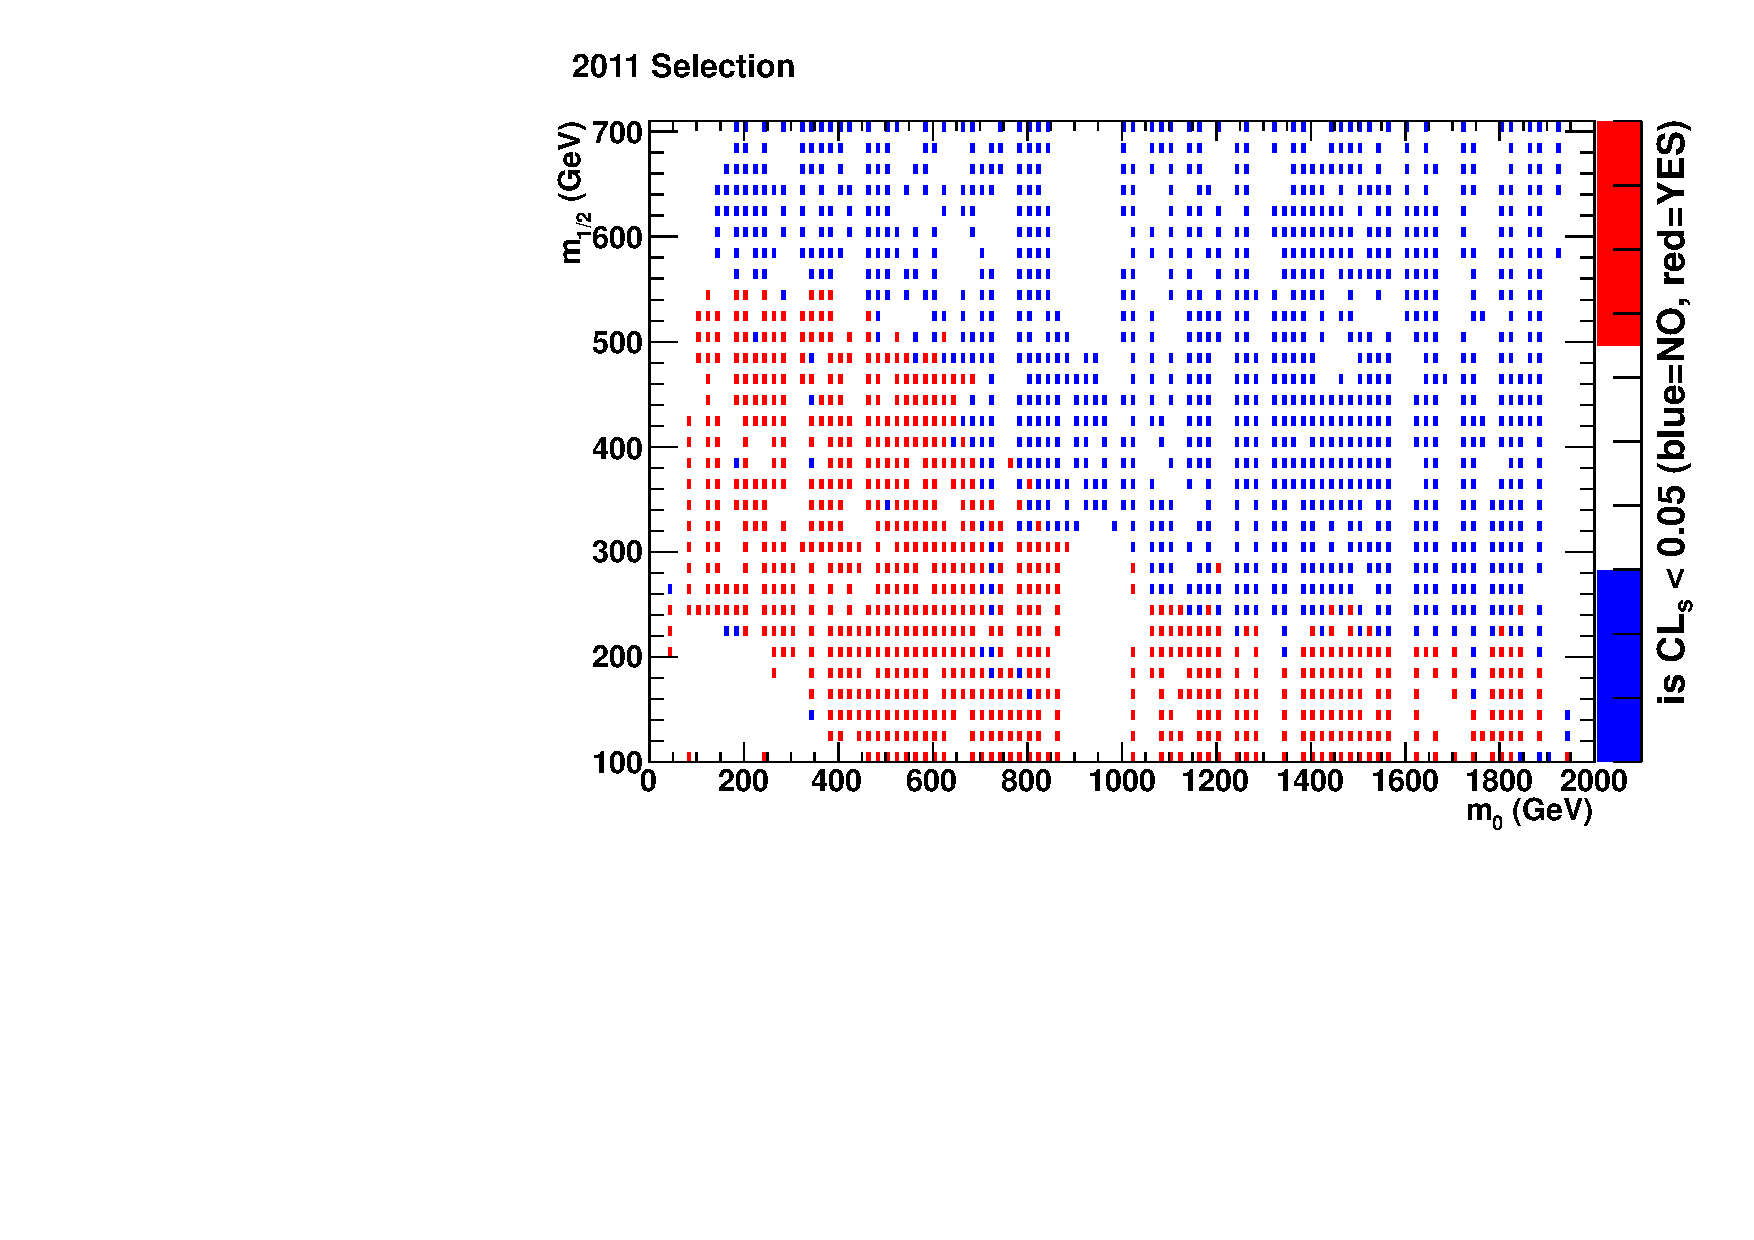
\includegraphics[width=0.49\textwidth]{Figures/RA4/AsWas_Modified_CLs}}
\subfigure[]{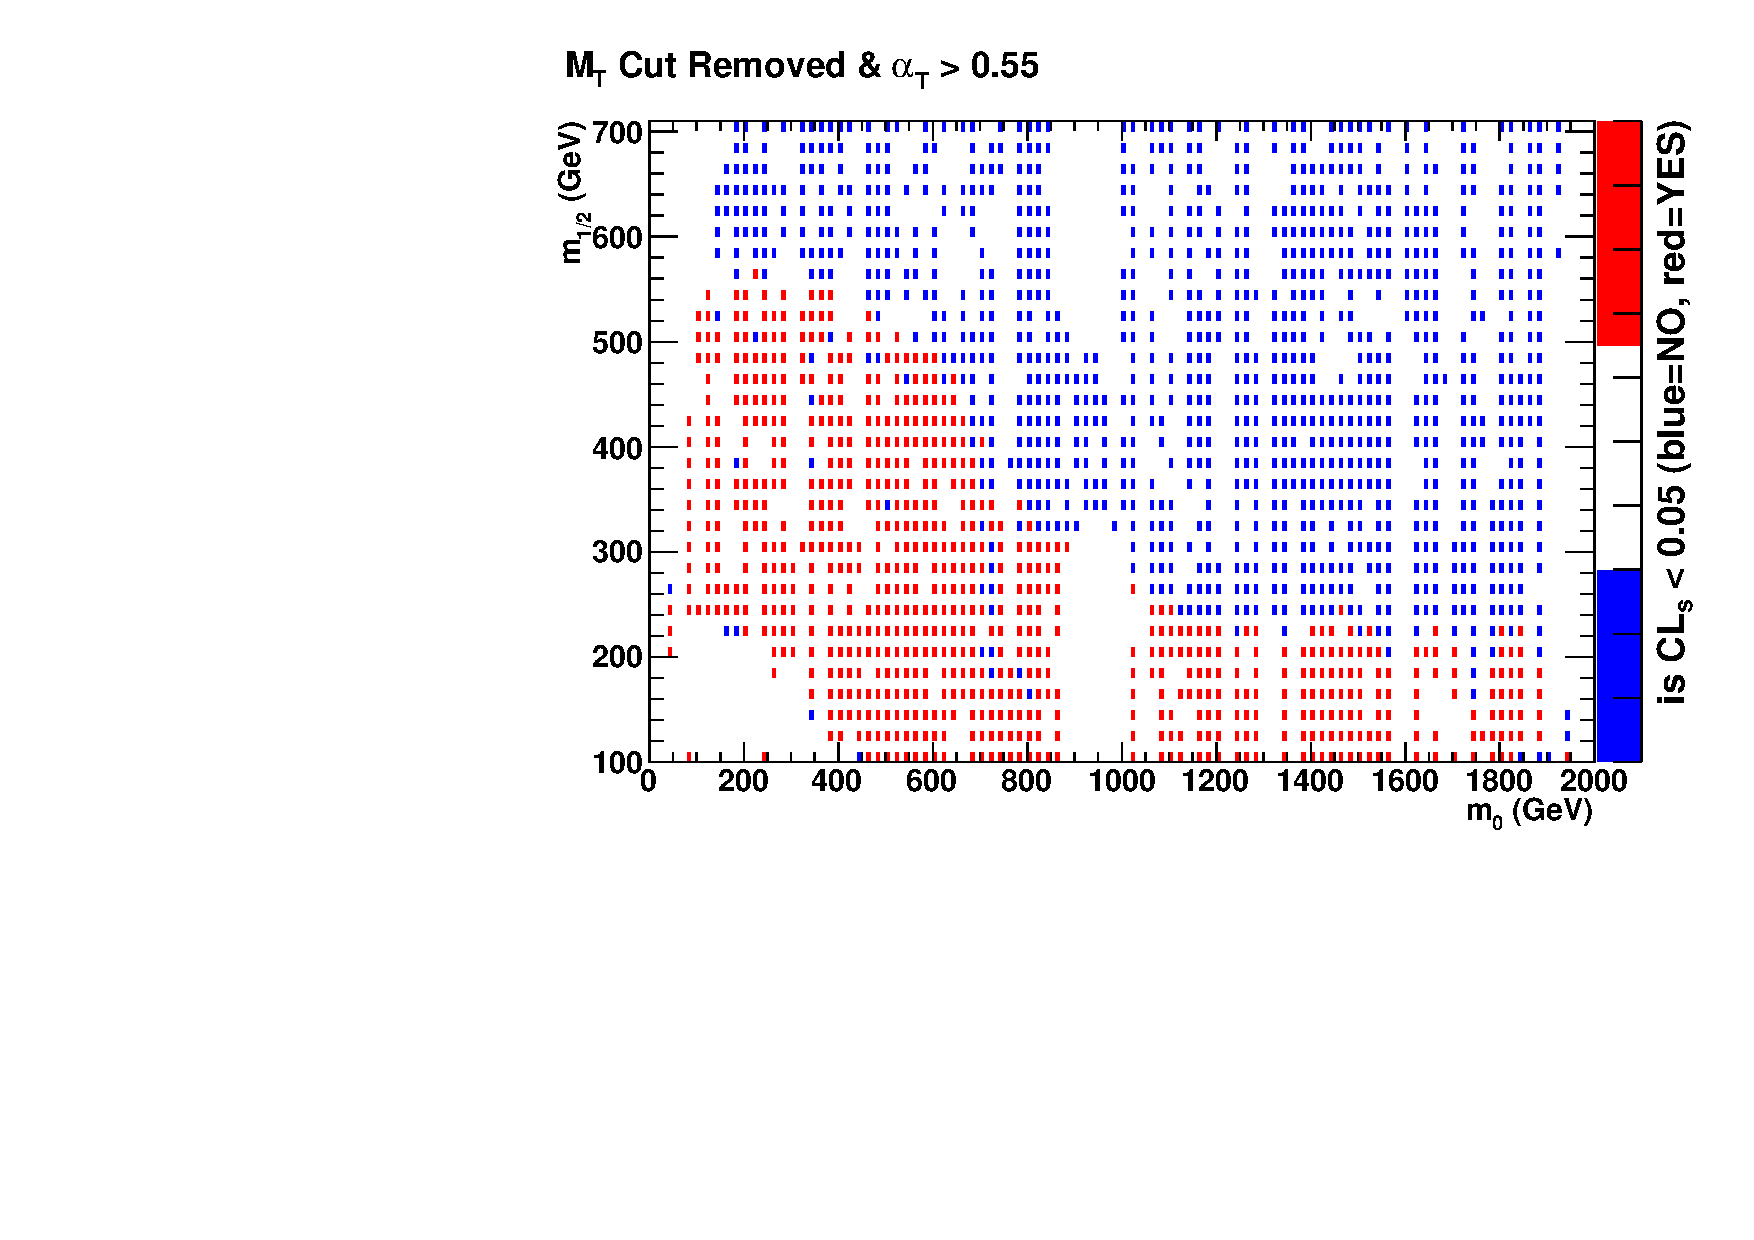
\includegraphics[width=0.49\textwidth]{Figures/RA4/hat_Modified_CLs}}
\subfigure[]{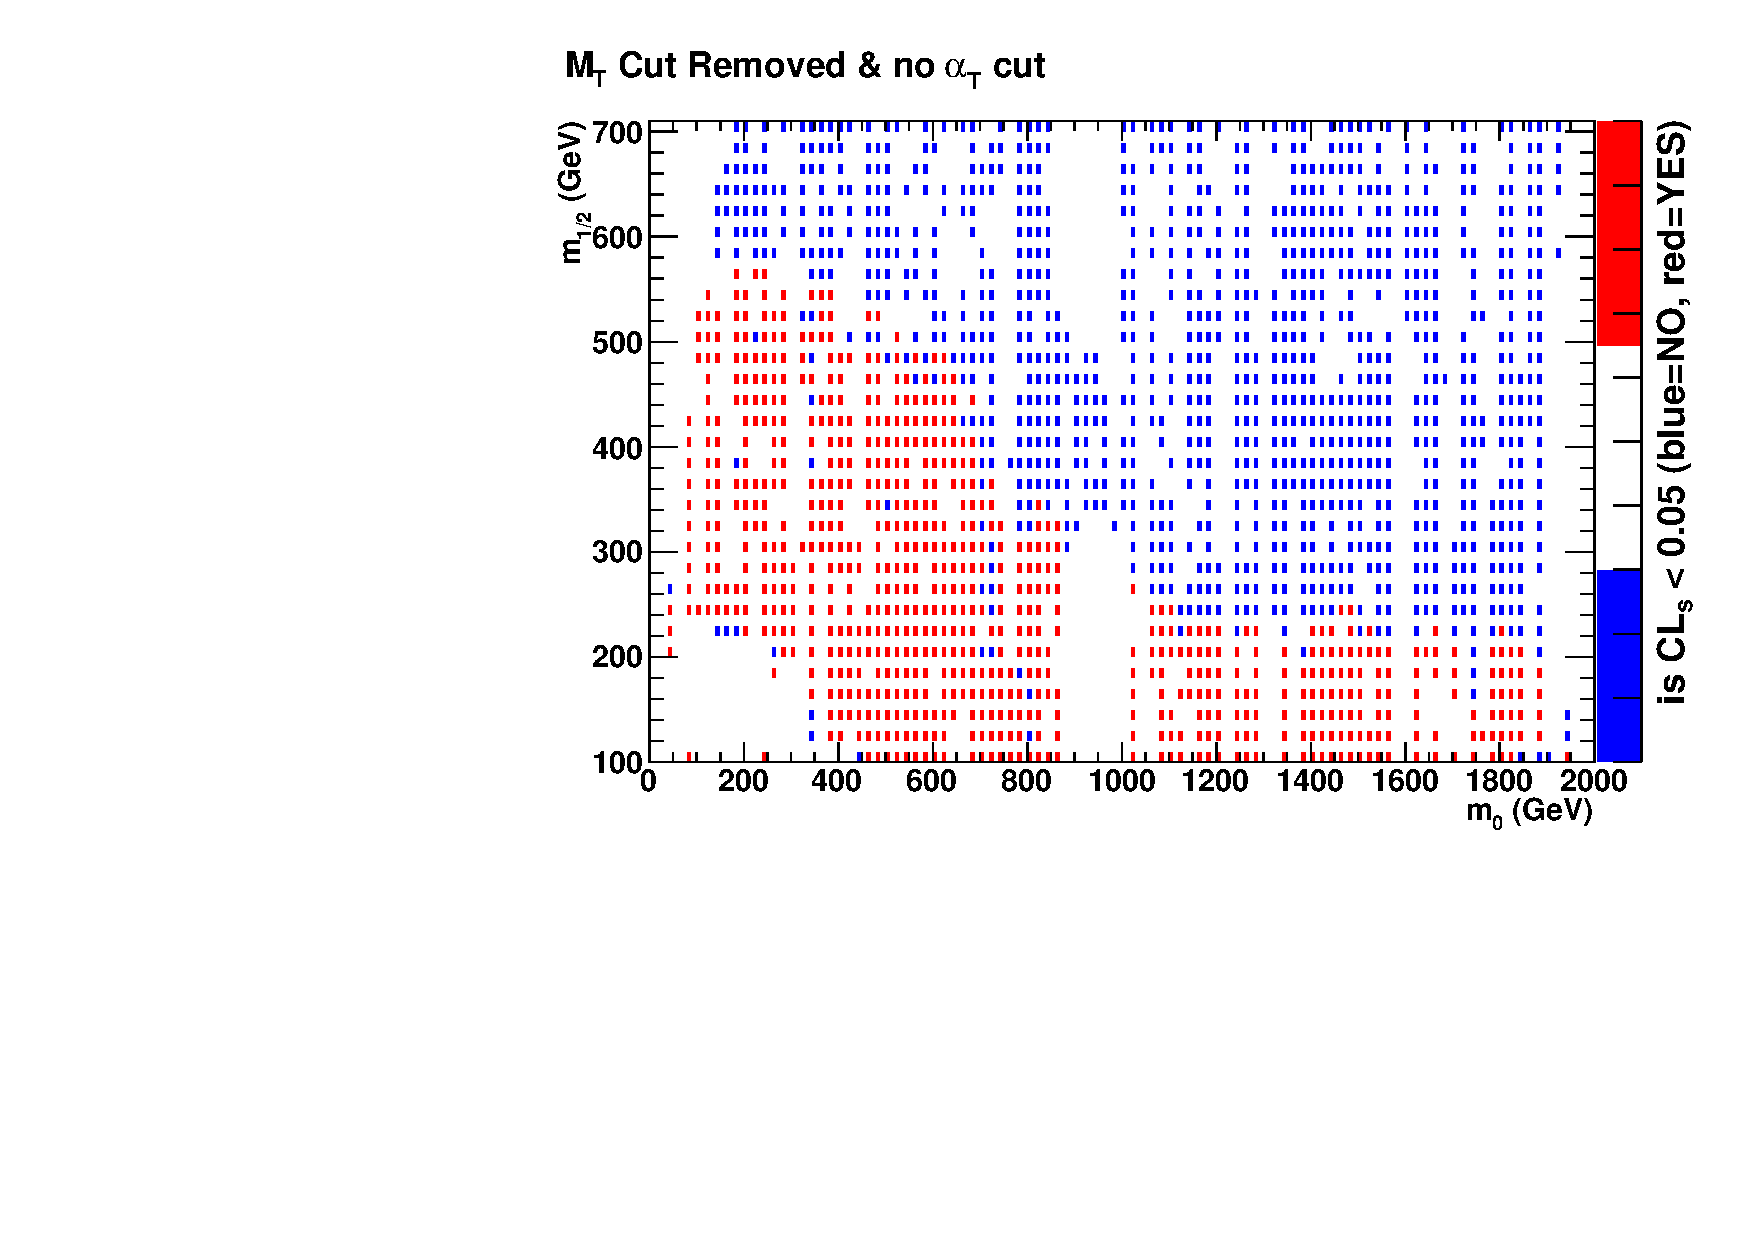
\includegraphics[width=0.49\textwidth]{Figures/RA4/noat_Modified_CLs}}
\subfigure[]{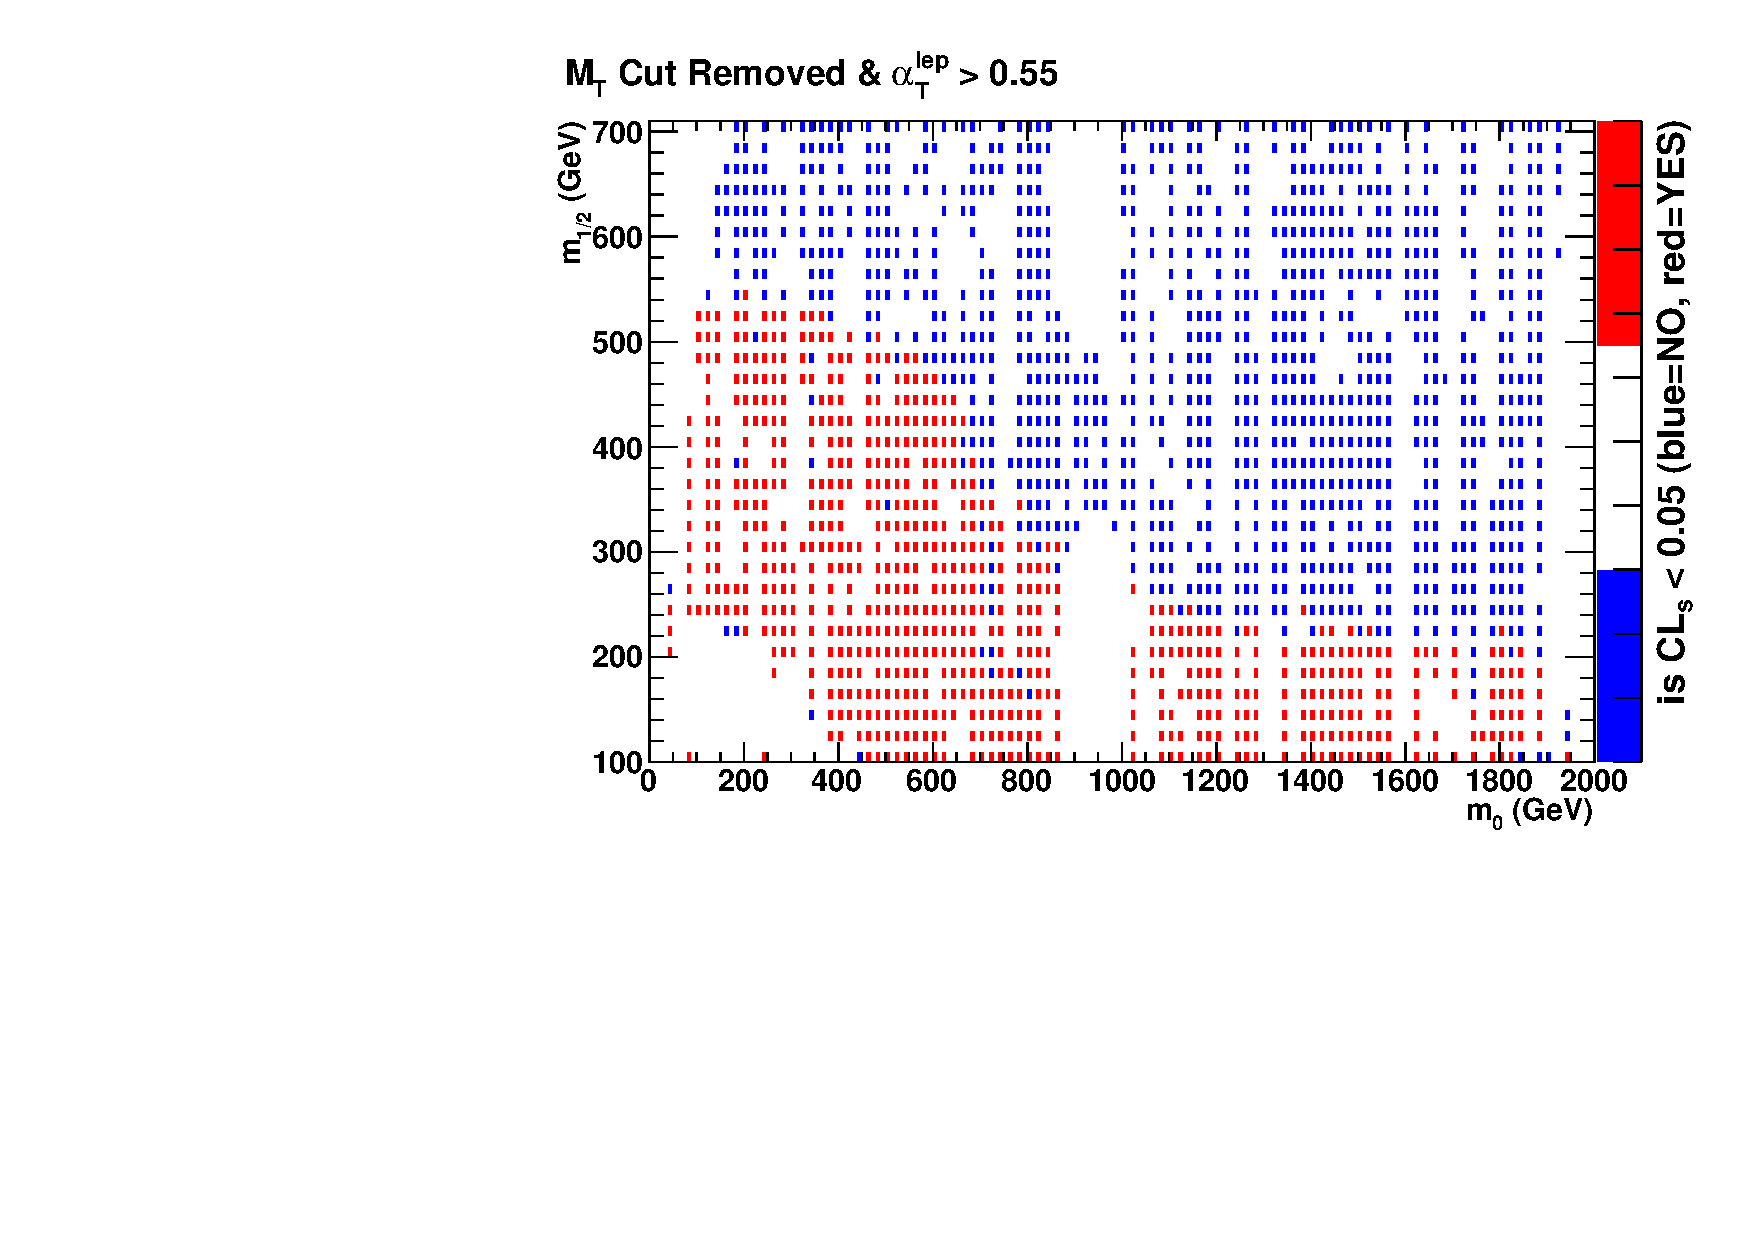
\includegraphics[width=0.49\textwidth]{Figures/RA4/lat_Modified_CLs}}
\caption{\label{fig:4fit}The CL$_{s}$ exclusion limit for the four different $\mu$ selection criteria, with CL$_{s}$ $<$ 0.05 shown in red (excluded at 95\% confidence) and CL$_{s}$ $>$ 0.05 shown in blue. Missing points are due to holes in Monte Carlo statistics. The 2011 Selection (a) is unchanged from Chapter~\ref{ch:ra1} and corresponds to the final limit plot there. The M$_{T}$ cut is removed for (a) with \alt $>$ 0.55, (b) with no \alt cut and (c) with \alt$^{lep}$ $>$ 0.55.}
\end{figure}









